\chapter{Proces uczenia}\label{chap:training}
{
    Do przetworzenia danych do wybranej postaci zostały wykorzystane modele wymagające uczenia.
    Ich opis został zawarty w sekcji \ref{chap:models_data_k} i \ref{chap:models_data_v}. Sekcja \ref{chap:main-model} oraz następujące
    poświęcone są opisowi procesu uczenia głównego modelu, czyli sieci neuronowej której 
    zadaniem jest ekstrakcja cech utworów treningowych.

    \section{Grupowanie wartości rytmicznych - k-Means}\label{chap:models_data_k}
    {
        Model k-Means został wykorzystany w celu wyznaczenia klastrów
        długości trwania dźwięków. Powyższy zabieg umożliwił ograniczenie wszystkich występujących 
        wartości rytmicznych do dyskretnego zbioru. 
        
        Model dzieli występujące przypadki na grupy w taki sposób, aby zminimalizować odległość 
        między przypadkami należącymi do jednej grupy.
        Do głównych parametrów tego modelu należy docelowa ilość klastrów, ilość iteracji
        oraz niezależnych uruchomień modelu mająca na celu rozwiązania problemu zatrzymywania uczenia w lokalnym minimum.

        Przykładowy wynik grupowania przedstawia rysunek \ref{grouping}.

        \begin{figure}[H]
            \centering
            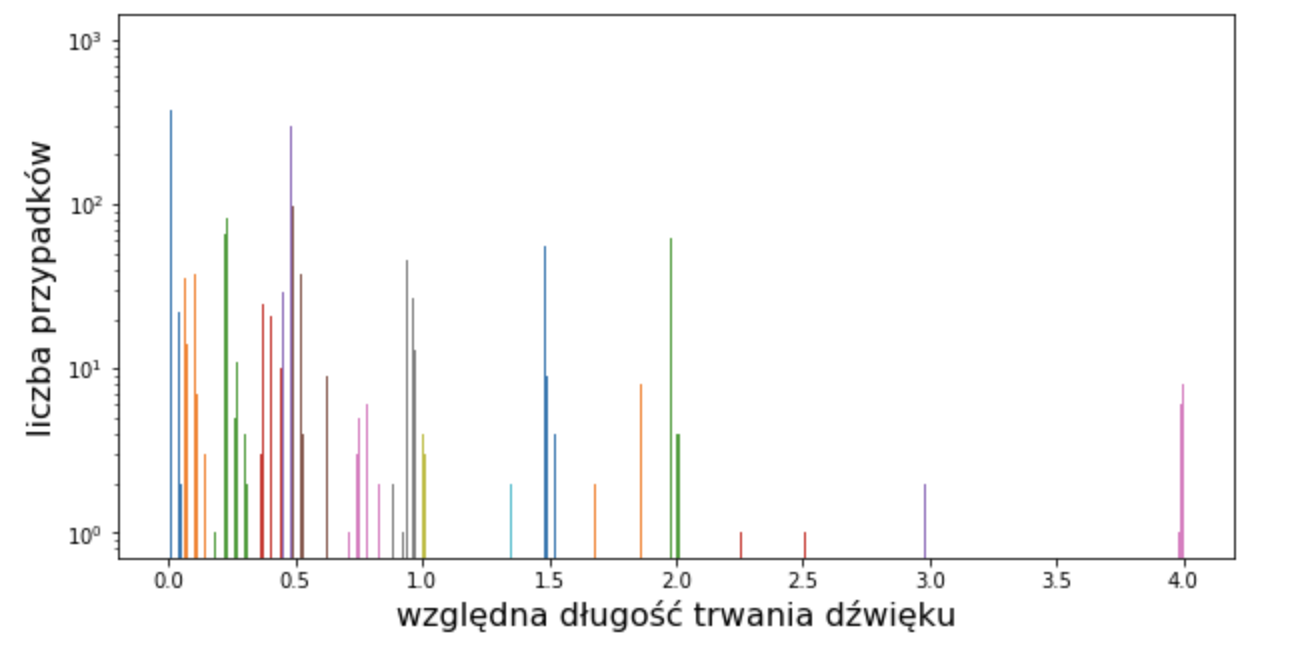
\includegraphics[scale=0.65]{grouping_grouped}
            \caption{Wykres przedstawiający rozkład długości trwania dźwięków oraz wynik grupowania. Dźwięki przydzielone do tej samej klasy są oznaczone tym samym kolorem.}
            \label{grouping}
        \end{figure}
    }

    \section{Wyznaczanie wektorów zanurzonych \\ - Word2Vec}\label{chap:models_data_v}
    {
        Kolejnym zastosowaniem uczenia maszynowego w etapie przetwarzania danych było użycie algorytmu Word2Vec. Algorytm 
        został użyty do wyznaczenia ciągłej reprezentacji rzadkich wektorów reprezentujących dźwięki.
        
        Uczenie algorytmu Word2Vec polega na wyznaczaniu wag ukrytej warstwy wielowarstwowego perceptronu
        uczonego wektorami reprezentującymi kolejne słowa należące do kontekstu.
        Model wymagał określenia docelowej wymiarowości wektorów i rozmiaru kontekstu. 

        Użycie powyższego modelu pozwoliło przekształcić  wektory kodu  M\,\,z\,\,N, gdzie M to ilość jednocześnie wybrzmiewających dźwięków a N to ilość wsystkich możliwych dźwięków, na wektory wartości ciągłych o wymiarze \(1 \times 20\).
    }
    
    \section{Architektura modelu sieci neuronowej}\label{chap:main-model}
    {
        Otrzymawszy dane w postaci sekwencji par wektorów opisujących dźwięki i ich czas trwania,
        przystąpiono do projektu architektury modelu. Z powodu dwuelementowej postaci danych
        zdecydowano się na zaprojektowanie modelu dwuwejściowego i dwuwyjściowego.

        Ponieważ charakter wektorów w sekwencji jest różny - wartości ciągłe opisujące dźwięki i 
        kategoryczny kod  1\,\,z\,\,N opisujący długość dźwięku - przed złączeniem wektorów postanowiono 
        przekształcić wektor  1\,\,z\,\,N przez warstwę gęstą o wymiarze mniejszym niż N. Celem tej operacji
        było wprowadzenie konieczności przez sieć kompresji informacji, co przełoży się 
        na wyznaczenie ciągłej reprezentacji kodu o mniejszej wymiarowości. 

        Następnie wektory zostają złączone, i ich sekwencje trafiają do warstw rekurencyjnej sieci LSTM, w której model ma szanse ekstrahować wiedzę o zależnościach między kolejnymi elementami sekwencji. W tym kroku analizowane są dane o wysokości i długości trwania dźwięków jednocześnie.

        Otrzymywane wektory reprezentacji ukrytej są połączone z osobnymi, 
        mniejszymi sieciami LSTM odpowiedzialnymi za przekształacnie reprezentacji 
        ukrytej zawierającej za równo informacje o wysokościach i długościach trwania dźwięków, 
        do postaci w której nacisk jest kładziony jedynie na jeden z dwóch powyższych aspektów. 
        Wektory otrzymywane na wyjściach osobnych sieci LSTM są przekształcane przez warstwy gęste będące wyjściami modelu. 
        Wspomniane przekształcenie przez warstwę gęstą umożliwia silniejsze uniezależnienie kodu 
        wyjściowego od wewnętrzej reprezentacji danych na których przeprowadzane są operacje 
        w sieciach rekurencyjnych, co pozostawia większą swobodę przy optymalizacji wag i wewnętrznej postaci danych.
        
        Celem wprowadzenia dodatkowych sieci LSTM do procesu uczenia modelu był podział zadania pozwalający na lepszą specjalizację modeli, które były uczone na podstawie jednej części danych w izolacji. Korzystnym efektem ubocznym tej operacji jest uzyskanie zaplanowanej struktury modelu dwuwyjściowego.

        Opracowaną strukturę modelu przedstawia rysunek \ref{model_struct}.
        
        \begin{figure}[H]
            \centering
            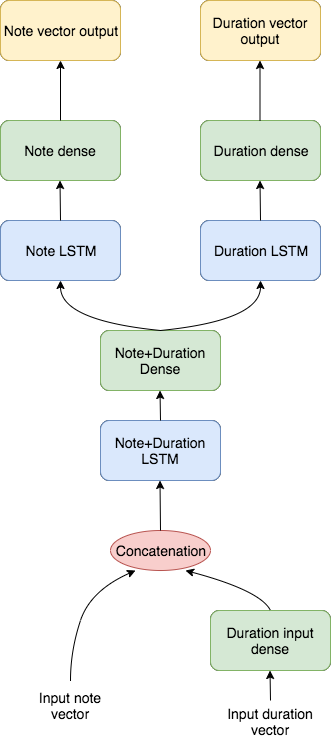
\includegraphics[scale=0.5]{model_struct}
            \caption{Diagram przestawiający architekturę modelu.}
            \label{model_struct}
        \end{figure}

        Z powodu różnego charakteru otrzymywanych wektorów, wyjścia modelu były uczone odzielnymi funkcjami błędu. 
        Wyjście odpowiedzialne za dźwięki uczone jest funkcją błędu odpowiednią do problemu 
        regresji - błędem średniokwadratowym, wyjście klasyfikujące długość dźwięku funkcją odpowiednią
        dla zadania klasyfikacji  1\,\,z\,\,N - kategorycznej entropii krzyżowej.
    }

    \newpage

    \section{Parametry modelu}
    {
        Podczas procesu uczenia najistotniejszymi parametrami były:
        \begin{itemize}
            \setlength\itemsep{-0.5em}
            \item rozmiar okna, czyli długość uczonych sekwencji,
            \item ilość przykładów w wiązce, czyli ile sekwencji było uczonych jednocześnie
            poprzedzając pojedyncze przeprowadzenie algorytmu propagacji wstecznej,
            \item rozmiar głównej sieci LSTM.
        \end{itemize}
    }

    \section{Proces uczenia}
    {
        Podczas uczenia modelu zdecydowano się na dynamiczny rozmiar okna,
        będący liczbą losową z zakresu <15, 50>. Motywacją tego wyboru były testowe 
        uruchomienia modelu potwierdzające zdroworozsądkową intuicję mówiącą, że większe wartości
        umożliwią uczenie dłuższych powtarzających się motywów, a krótsze wartości umożliwią uczenie lokalnego następstwa nut.

        Dodatkowo, warto przybliżyć sposób tworzenia przypadków testowych. Naiwnym podejściem byłoby
        jednokrotne utworzenie zbioru danych poprzez utworzenie wszystkich możliwych podciągów o zadanej
        długości (rozmiarze okna) i dalsze używanie ich jako statycznej listy przypadków. 
        Takie rozwiązanie nie umożliwiałoby dynamicznej zmiany długości sekwencji, i wymagałoby dodatkowego 
        kroku w procesie przetwarzania danych. Alternatywnym podejściem, na które się zdecydowano jest dynamiczne
        wybieranie losowych podciągów z utworów należących do zbioru danych, które odbywa się równolegle z uczeniem modelu. 
        Główną obawą jaką można posiadać do takiego podejścia jest jego narzut czasowy podczas uczenia modelu, 
        aczkolwiek zaobserwowano że tempo przygotowania i kolejkowania kolejnych przypadków testowych znacznie przewyższa tempo ich uczenia.

        % \bigskip

        Podczas testowania różnych wartości pozostałych parametrów, zaobserwowano interesujący wpływ ilości przykładów w wiązce.
        %%% można jakby co opisać czym jest wiązka 
        Większe wartości, rzędu 16 lub 32 miały negatywny wpływ na jakość generowanych sekwencji. 
        Mniejsze wartości prowadziły do przetrenowania modelu.

        Rozmiar głównej sieci miał spodziewany efekt, zbyt duży prowadził do przetrenowania. Dla obecnego
        zbioru danych zdecydowano się zachować wartość 64 jednostek.

        % \bigskip

        Podczas uczenia monitorowano metryki opisujące jakość predykcji i postęp uczenia modelu.
        Do mierzonych metryk należą funkcje błędu dla poszczególnych wyjść modelu, średni błąd kwadratowy
        wyjścia reprezentującego wektory dźwięków oraz kategoryczna dokładność stwierdzająca czy najwyższa wartość
        wektorów znajduje się na tym samym indeksie.
        
        Proces uczenia podzielone był na epoki. W klasycznych zastosowaniach przez jedną epokę rozumie się jednokrotne
        wykorzystanie każdego przykładu z zbioru treningowego. Jednakże z powodu opisanego powyżej sposobu otrzymywania
        przypadków testowych, niemożliwe było wykorzystanie tej definicji. Zdecydowano się na arbitralne przyjęcie konkretnej 
        ilości przypadków testowych jako jednostkę jednej epoki. Obraną wartością był jeden tysiąc.

        Po ukończeniu każdej epoki przeprowadzane były pomiary skuteczności modelu na danych wyjętych spoza korpusu 
        danych treningowych. Ponieważ problematycznym byłoby wydzielenie sekwencji walidacyjnych z części środkowych
        utworów, zdecydowano się zarezerwowanie ostatnich 25 elementów sekwencji z każdego utworu.
        Na podstawie wyników powyższych miar, można wyciągać wnioski dotyczące postępu uczenia modelu.

        Uczenie zaplanowano na okres 35 epok, co przełożyło się na czas bliski 20 minut. Dobrana ilość epok wynikała 
        z obserwacji spadku trafności predykcji następującej po tej liczbie powtórzeń. Do uczenia wykorzystano
        akcelerację sprzętową w postaci karty graficznej dostępnej w usłudze chmury obliczeniowej Google Colab.

        Rysunki \ref{epoch_val_duration_output_categorical_accuracy_} i \ref{epoch_val_notes_output_mean_squared_error_} zawierają wykresy opisujące miary postępu uczenia podczas kroków walidacyjnych. Na wykresy naniesiono krzywe wygładzające wartości pomiarów w celu wyraźniejszego ukazania występujących tendencji.

        \begin{figure}[H]
            \centering
            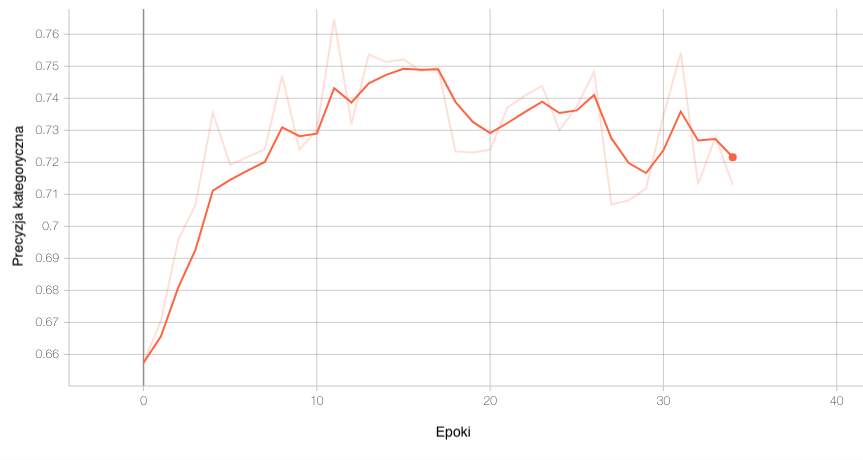
\includegraphics[scale=0.5]{epoch_val_duration_output_categorical_accuracy_}
            \caption{Wartości miary precyzji predykcji długości trwania dźwięków}
            \label{epoch_val_duration_output_categorical_accuracy_}
        \end{figure}

        \begin{figure}[H]
            \centering
            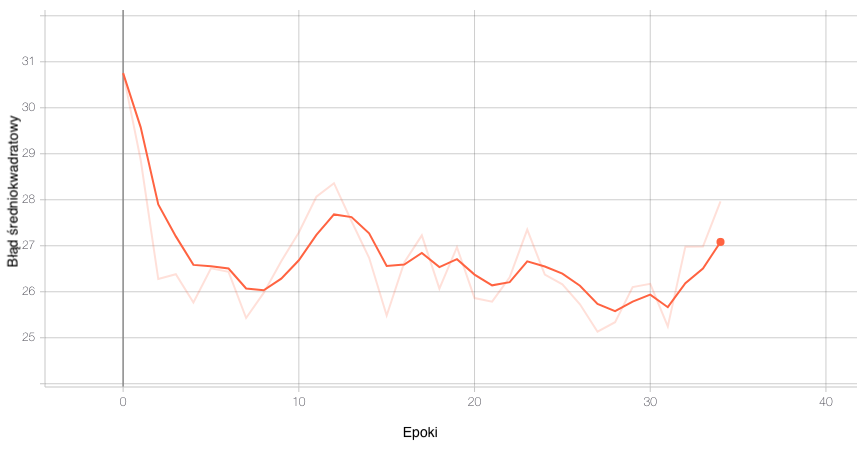
\includegraphics[scale=0.5]{epoch_val_notes_output_mean_squared_error_}
            \caption{Wartości błędu średniokwadratowego predykcji wektora dźwięków}
            \label{epoch_val_notes_output_mean_squared_error_}
        \end{figure}

        Na rysunkach można dostrzec trafność predykcji klasy długości trwania dźwięku, oraz błąd średniokwadratowy
        predykcji wektorów dźwięków. W pierwszej połowie uczenia na obydwu wykresach można zaobserwować pożądaną tendencję,
        czyli wzrost trafności i spadek błędu. Po kolejnych epokach postęp uczenia malał, lub nawet zachodził jego regres.
    }

    \section{Generowanie próbek}
    {
        Opierając się na założeniu, że wyuczony model posiada pewną wiedzę możliwe jest przejście do procesu generowania próbek.

        \subsection{Opis podejścia}\label{sec:gen_method}
        {
            Proces otrzymywania generowanych sekwencji zależny jest od rodzaju modelu.
            W przypadku modeli typu sequence-to-sequence, możliwe byłoby podanie losowego 
            wektora na część modelu w którym dokonuje się przekształcenie jednowymiarowej postaci ukrytej na sekwencję.
            Przy zastosowaniu architektury opisanej w poprzednim rozdziale, konieczne będzie 
            rozpoczynanie generacji sekwencją, dalej nazywaną ziarnem. 

            Ponieważ opracowany model przekształca sekwencje danych wejściowych na sekwencje
            o tej samej długości, sekwencja otrzymana po zadaniu ziarna będzie tej samej długości.
            Proponowanym rozwiązaniem tego problemu jest łączenie sekwencji wejściowych z sekwencjami wyjściowymi,
            i ponowne wprowadzenie jej do sieci. Krok ten jest powtarzany aż do otrzymania sekwencji o pożądanej długości.
        }

        \subsection{Opisy ziaren}
        {
            Kolejną kwestią, którą rozważono, jest opracowanie sposobów generowania ziaren.
            Oczywistym pomysłem jest zastosowanie wektorów o wartościach zerowych lub losowych.
            Ponadto, opracowano ziarna zawierające pojedynczy dźwięk, sekwencję losowych dźwięków
            i sekwencję dźwięków często współwystępujących. Dźwięki współwystępujące są obierane poprzez
            porównanie odległości między składowymi ich wektorów i wybranie wektorów o zbliżonych składowych.
        }
    }
}